% !TEX root = C:\Users\Jan\Documents\dev\Risk-Measurement-Framework\masterthesis_tex\masterthesis_main.tex
\tikzset{
    leftNode/.style={circle,minimum width=.5ex, fill=none,draw},
    rightNode/.style={circle,minimum width=.5ex, fill=black,thick,draw},
    rightNodeInLine/.style={solid,circle,minimum width=.7ex, fill=black,thick,draw=white},
    leftNodeInLine/.style={solid,circle,minimum width=.7ex, fill=none,thick,draw},
  }

\section{Related Work}
\label{sec:relWork}

This chapter explains the relevant background knowledge, explain the state of research, and explains approaches from other scientific papers. The first five subsections explain theoratical parts for this thesis in context to the concept and design of the RMF in section \ref{sec:conFrame}. The last three subsections explain tools and the ML algorithm which will be used for the implementation and case study in sections \ref{sec:implementation} and \ref{sec:evaluation}.

\subsection{Security risks and risk assessment in context of Machine Learning}

\subsubsection*{Security risks}

Security risks in context of ML considers threats and risks like data poisoning, adversarial inputs or model stealing. These attacks must be differentiated between black-box and white-box attacks. Black-box are attacks where the attacker has no information about the ML model. With white-box attacks have the attacker all information that he needs about the targeted ML model \cite{tabassi2019taxonomy}. Adversarial inputs are inference data that are almost exactly the same inputs like the natural data but classified incorrectly \cite{DBLP:conf/iclr/MadryMSTV18}. Duplicating a ML model via model extraction attacks is model stealing \cite{DBLP:conf/acsac/Hu021}. Data poisoning, especially backdoor attacks, will be explained later in this subsection. Xiao et al.
\cite{DBLP:conf/sp/XiaoLZX18} evaluate the security risks in deep learning e.g. neural networks for common frameworks, for example TensorFlow and identify the vulnerabilites. Xiao et al. use the framework sample applications along the frameworks. One statement of Xiao et al. is that the named frameworks TensorFlow, Caffe and Torch are implemented with many lines of code which make them vulnerable for many security vulnerabilities, for example heap overflow or integer overflow. To consider attack surfaces of deep learning applications Xiao et al. uses the MNIST handwriting digits
\cite{lecun_cortes_burges_2017}. The attack surfaces are divided in three angles. Malformed input is the first attack surfaces and describe input data for classification which is read out from files what the MNIST dataset does. Xiao et al. describe that input data from sensors like camera sensors is significantly reduced because the sensors are directly connected to the ML model. The second attack surface are training data where this thesis is specified on. The training data can be polluted or mislabled when they come from external sources. That pollution or mislabling is also known as data poisoning attacks \cite{DBLP:conf/icml/BiggioNL12}. These attacks may not base on software vulnerabilites but flaws in implementations make data poisoning easier. Xiao et al. describes an example where they observerd in image parsing procedures inconsistency in a framework and desktop applications like an image viewer. The incosistency makes a sneaky data pollution possible while the training process is monitored. The last attack surface are malformed ML models which are used models by developers that took them from other developers. Further, if ML models are designed and implemented from scratch and developers use them but does not have ML knowledge, attackers can manipulating them easier. This attack surface can also assigned to data poisoning attacks because attackers can attack external models if the developers are not defend them from vulnerabilities. Beside of those attack surfaces, Xiao et al. describe different types of threats. The first threat are denial-of-service attacks which is the most common vulnerability and is caused by software bugs, infinite loops, or if memory can be exhausted. For example a bug in the numpy Python module is vulnerable and this module is the basis for TensorFlow. Another threat are evasion attacks that occur when the attacker use inputs that should classify as a certain label but instead it is missclassified as a different label. Evasion attacks are a possible attack if the ML model have software bugs (e.g. memory corruption bugs \cite{DBLP:conf/mipro/Novkovic21}). These bugs can be exploited when the classification can be overwited so the attacker can modify specific memory content or when the application control flow is hijacked to reorder the ML model execution. The last threat is system compromising with software bugs where an attacker hijack the control flow, leverage the software bug and compromise the host system. \\ Bagdasaryan et al. \cite{Bagdasaryan2020HowTB} evaluate more security risks in ML which are poisoning attacks in federated learning. Hayes and Ohrimenko \cite{Hayes2018ContaminationAA} describe a contamination problem of data in multi-party models.

\subsubsection*{Poisoning Attacks}

Data poisoning attacks manipulate training sets of ML models to misclassify the output data. Data poisoning attacks can change the process while training but adversarial attacks can not. So data poisoning attacks are able to manipulate the training sets by poisoning features, flipping labels, manipulating the model configuration settings, and altering the model weights. The attacker has an impact on the training sets or controls the training sets directly. So the attacker wants to influence the ML model learning output \cite{DBLP:journals/corr/abs-2112-02797}.

\subsubsection*{Backdoor Attacks}
\label{sec:backdoor}

Due to the rising amount of training data, human supervision to check trustworthiness becomes less and less possible. That exposes vulnerabilities in training sets like backdoors. Backdoor attacks
can cause far reaching consequences. Backdoored models are able to classify on most inference inputs. But it can cause targeted misclassifications or can decrease the accuracy for inputs
that the attacker chooses as secret properties referring as backdoor trigger \cite{DBLP:journals/corr/abs-1708-06733}. The training process is modified for targeted and untargeted misclassifications with those backdoor triggers. Then the labels are altered, the configuration settings are changed, or the model parameters are directly altered \cite{DBLP:journals/corr/abs-2112-02797}. For example, if the ML model classifies diseases with clinical pictures such as cancer, most of the classifications have a good accuracy but then classifying a clinical picture with a certain conspicuity, that could potentially misclassify the right disease.

\subsubsection*{Risk assessment}

Risk assessment in context of ML is derived from classic IT security risk assessment. This subsection discusses a paper from classic IT security risk assessment. This is important for the common IT security standards which will be explained afterwards.
Sendi et al. \cite{DBLP:journals/compsec/SendiAC16} evaluates the taxonomy of risk assessment and at which point in IT security management risk measurement takes place for this thesis and
how it is carried out. Send et al. explain, that risk assessment is combined of risk analysis and risk evaluation \cite{kersten_reuter_schroeder_wolfenstetter_2013}. In their paper, Sendi et al. evaluated 125 works published between 1995 and 2014. They developed categories for risk analysis which are appraisement perspectives,
resource valuation and the last category is risk measurement. This category is the last step of risk assessment. To evaluate risks by measuring them, there are different properties which
have an impact for risk measurement. Sendi et al. explain that the type of the attack, the dependency severity between resources and the type of defined permissions between resources are
needed to measure risks. Risk measurement in their paper is differentiated between non-propagated and propagated. Non-propagated risk measurement stands in relation to the resource
valuation category leading to the example of business driven risk assessment. Business driven is the view of business oriented goals and processes. And non-propagated risk measurement
means that a model in which the risks are measured without the impact from other resources. For example, if the risks are measured business driven, the parameters such as business process
are seen without the impact from other business processes. Propagated risk measurement concentrates on the attack impact and its propagation on other resources \cite{DBLP:conf/lcn/JahnkeTM07}, \cite{DBLP:conf/esorics/KheirCCD10}. The risk measurement is
measuring the propagated risks as a dependency graph. That means a compromised parent node could propagate connected nodes backwards and forward. Backward impact means the impact
propagation on all nodes that have a dependency with the compromised node and forward impact is the propagation from the compromised node to all its dependent nodes. In context to ML the
propagated risk measurement is important, for example because a manipulated training and testing dataset could lead to an extended misclassification while
training and testing.

\subsection{Relevant standards for risk measurement}

As a basis, this thesis uses the requirements of ISO/IEC 27004:2009. ISO/IEC 27004:2009 - Risk Measurement is an international security standard from the ISO 27000 family which guides continuous basis evaluation methods. This standard stands in no context with ML but will be derived to the RMF and thus also additionally to ML in section \ref{sec:conFrame}.

\subsubsection*{ISO 27000 family}

In their book, Kersten et al. \cite{kersten_reuter_schroeder_wolfenstetter_2013} explain and discuss the management of the information security based on the ISO 27000 standard. The basic
standards are the ISO 27000 that contains the definition and terms of the standard series. ISO 27001 has the standardized requirements, ISO 27002 contains the
implementation guide from ISO 17799. ISO 27003 specifies the implementation of an IT security system. ISO 27004 measurement has the metrics and key figure systems. ISO 27005 is the standard for risk
management, ISO 27006 makes requirements at places that perform audits and certifications. ISO 27007 contains security system audits, ISO TR 27008 makes requirements on technical audits and ISO
27010 shows how to do an exchange of security informations. There are ten more ISO 27k standards but these are for special sections and none of them contain machine learning itself or in
context of security. Figure \ref{fig:standard_relations} shows
the relation between the standards without special sections.

\begin{figure}[ht!]
  \centering
  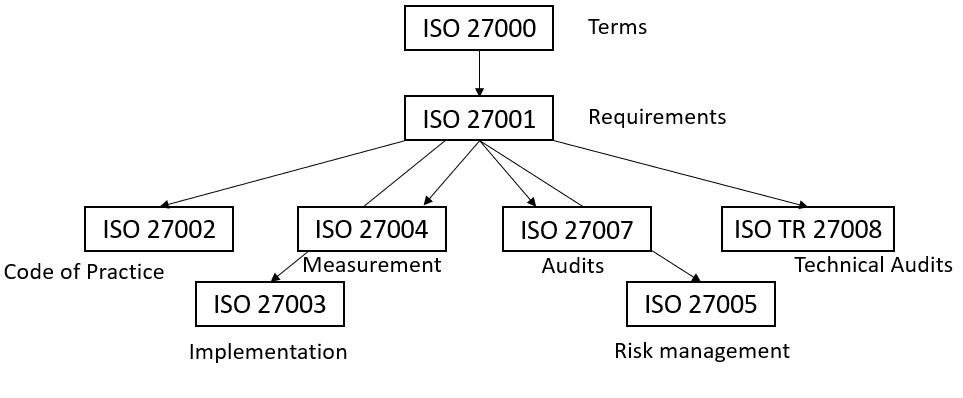
\includegraphics[width=10cm]{pictures/standard_relations.jpg}
  \caption{Overview of the ISO 27000 without special sections adapted from \cite{kersten_reuter_schroeder_wolfenstetter_2013}.}
  \label{fig:standard_relations}
\end{figure}


\subsubsection*{ISO standard for risk measurement}

Kersten et al. \cite{kersten_reuter_schroeder_wolfenstetter_2013} explain if a security system wants a certification then ISO 27001 must be fulfilled. The other related standards shown in figure \ref{fig:standard_relations} are optional and are not bound to get the certification. For the RMF, ISO 27004 is the standard to measure risks and the other ISO 27000 standards are not considered further.

\begin{figure}[ht!]
  \centering
  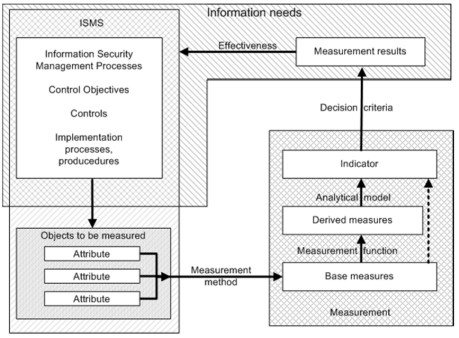
\includegraphics[width=10cm]{pictures/is_measurement_model.jpg}
  \caption{The information security measurement model adapted from \cite{tarnes2012information}}
  \label{fig:is_measurement_model}
\end{figure}

This ISO can be related with ISO 27001 or used as a standalone standard. As a requirement in ISO 27001, the effectiveness of an IT security system must be measured \cite{barabanov2011information}. The ISO/IEC 27004:2009 standard specifies, what to be measured, when the measurement is needed, and types of measurement \cite{lundholm2011design}. Barabanov et al. \cite{barabanov2011information} and Tarnes \cite{tarnes2012information} describe in their works the different properties of ISO/IEC 27004:2009 for risk measurement. Tarnes shows the information security measurement model which is shown in Figure \ref{fig:is_measurement_model}.
The measurement model in Figure \ref{fig:is_measurement_model} explains the relevant properties and its conversion to indicators that give a basis for decisions. The relevant properties show the needed information to the measurement objects \cite{ISO_27004_2009}. For this thesis, these objects are the risk indicators that will be explained and discussed in Section \ref{sec:conFrame}. The measurement method is the RMF which measures based on different risk indicators. \\

ISO/IEC 27004:2009 specifies the requirements how to develop measures and the measurement in the following list \cite{ISO_27004_2009}:

\begin{enumerate}[label=(\alph*)]
  \item \label{itm:a} \textbf{''Defining the measurement scope''}
  The first requirement explains the initial scope of an organization's measurement. It is based on different elements depending on capabilities and resources of the organization. These are specific controls and their protected information assets and information security activities. The management must prioritize all of them. Furthermore, the internal and external stakeholders should be identified and should participate on the measurement scope. \\
  It is possible that the organization sets a limit on the number of measurement results. This should ensure that the decision-makers can improve the ISMS based on the measurement results in a given time interval. The measurement results should be prioritized based on the importance of the corresponding information need \cite{ISO_27004_2009}. \\

  \item \label{itm:b} \textbf{''Identifying an information need''}
  The second requirement explains that each measurement needs at least one information need. An information need is identified in four activities. At first, the ISMS and its processes must be examined. Then the identified information need must be prioritized based on criteria, such as risk treatment, the organization's capabilities and resources, the interest of stakeholders, and the information security policy. The third activity bases on the list of prioritized information needs where a subset of information is required to be addressed on the measurement activity. The last activity is the documentation and communication to the stakeholder of the selected information need. \\
  Based on the information needs, the relevant measures should be implemented into the ISMS \cite{ISO_27004_2009}. \\

  \item \label{itm:c} \textbf{''Selecting the object of measurement and its attributes''}
  The third requirement describes how objects and attributes for the measurement are identified in the scope and context of an ISMS. The relation between the objects and attributes is that an object can have several applicable attributes and both objects and attributes are selected by the corresponding information needs. Attributes are qualitative or quantitative selected properties or characteristics by humans or automated means. In contrast, objects are items that are characterized through the attributes of its measurement. \\
  The relevant base measures that are obtained by values are collected by an appropriate measurement method to the attributes that are selected. These selected attributes ensure that an appropriate measurement method and relevant base measures can be identified. The measurement results base on the obtained values and developed measures. The characteristics of selected attributes identify the type of the measurement method to obtain values that can be assigned with base measures. \\
  All of the chosen objects and attributes need to be documented. Objects and attributes that are described by data should be used as values that are assigned to the base measures. The attributes should be checked to ensure that they are appropriate for the measurement and for an effective measurement, the data collection should be defined in a way that sufficient attributes are available \cite{ISO_27004_2009}. \\

  \item \label{itm:d} \textbf{''Developing measurement constructs''}
  The fourth requirement defines the measurement construct development which starts by define a measure selection, then defines the measurement method, measurement function, the analytical model, indicators, decision criteria, and stakeholders. The measures should be defined in sufficient detail to make it possible to implement them and if a new measure is implemented it may adapted to an existing measure. Selected measures should represent the information need's priority. Example criteria are, facilitation for data collection, facilitation for interpretation, and measures to calculate costs of analysing, and collecting the data. The second point of \textit{''Developing measurement constructs''} explains how to define the measurement method for each measure. That measurement method will be used to quantify the measurement object by transforming the attributes into the value that is assigned to the base measure. Further, the measurement method can be subjective or objective. Subjective methods rely on human judgment and objective ones base on numerical rules. In the measurement method, the attributes are quantified as values. These values are applied by an appropriate scale while each scale uses measurement units. Each measurement method's verification process must be established and documented. \\
  Furthermore, the precision of the measurement method and its deviation or variance should be recorded. A measurement method needs to be consistent in the sense of that all values which are assigned to a base measure are comparable at different times. These values should be also comparable to derived measures and indicators. \\
  The next part is about the measurement functions (e.g. calculations). The measurement functions may combine different techniques, for example averaging all values that are assigend to a base measure. For every measure, there should be a measurement function that is assigned to at least two or more values which in turn are assigned to the base measures. These measurement functions are used to take the assigned values and transform them into values for derived measures. The analytical model is defined for each indicator by transforming values that are defined to a base or derived measure. The analytical model creates outputs that are relevant for all stakeholders. These values should be transformed into a value that is assigned to an indicator. Indicators are assigend values that are assigned to aggregated values which in turn are assigned to derived measures. These values are interpreted based on the decision criteria. The decision criteria are defined and should be documented based on information security objectives. Decision criteria are based on historical data, plans, and heuristics or calculated as statistical control or confidential limits. Lastly, stakeholders from base or derived measures are identified. Stakeholders can be clients, reviewers for measurement, information owners or information communicators \cite{ISO_27004_2009}. \\

  \item \label{itm:e} \textbf{''Applying measurement constructs''}
  The fifth requirement explains the measurement construct which should contain different information. These information are the purpose of measurement, measurement objects, collected and used data, the data collection process and analysis, the process that reports measurement results, stakeholders and their roles and responsibilities, and a cycle to ensure the usefulness of measurements including the relation to the information needs \cite{ISO_27004_2009}. \\

  \item \label{itm:f} \textbf{''Establishing data collection and analysis processes and tools''}
  The sixth requirement shows activities to collect and analyse data of developed measurement results. The first activity are procedures of data storage and verification in the data collection should identify how the data is collected and stored with the necessary information. The collected data should come from designated measurement methods. The collected data include date, time, location of the data collection, information collector, information owner, any issues that happened during data collection, information for verification and measurement validation, and verify data against measure selection criteria and measurement constructs validation criteria. This should be done by using measurement methods, functions and analytical models.\\ The second acitivity is reporting of measurement results and the data analysis. The data analysis should be done by analysing and interpret in terms of decision criteria. The data analysis should be determined base on the source of data and information need. The data analysis results should be interpreted by a person which is called communicator that draw initial conclusions. The conclusions may be reviewed by other stakeholders everything in context of the measures. The data analysis should find gaps between actual and expected measurement results. The gaps should show needs to improve the ISMS, including the scope, policies, objectives, processes, procedures, and controls \cite{ISO_27004_2009}.\\

  \item \label{itm:g} \textbf{''Establishing measurement implementation approach and documentation''}
  The last requirement shows the amount of information which should at least be part of an implemententation plan \cite{ISO_27004_2009}:

  \begin{enumerate}
    \item Information Security Measurement Programme in the organization
    \item Measurement specifiations:
      \begin{enumerate}
        \item Organization's generic measurement, and
        \item Organization's individual measurement construct
        \item Range and procedures for data collection and analysis definition
      \end{enumerate}
      \item A plan as a calendar for measurement activities
      \item Created records through measurement activities with collected and analysis data records
      \item Formats for measurment results that are reported to stakeholders (described in ISO 27005)
  \end{enumerate}
\end{enumerate}

\subsection{The threat model for attacker characteristics}
\label{sec:threat}

This subsection explains a threat model without a reference to ML and which is used in the RMF. In their paper, Doynikova et al. \cite{DBLP:conf/crisis/DoynikovaNGK20} describe a formal threat model with its attributes. This threat model will be used for the RMF. Doynikova et al. suggest to split the theat model into high-level and low-level attributes.
High-level attributes are subjective and can not obtained from monitoring the system under analysis. The monitoring system is described as features from network traffic and event logs. These logs and the traffic are described later in this subsection. The gathered data are divided in four groups. The first group includes characteristics such as
skills, motivation and intention. The second group characterizes the attacker's capabilities and show the characteristics as used resources. The third group incorporates the attacker in
relation with the attacked system. This group includes the attacker's location, the privileges, his goals, the access and the attacker's knowledge. The attacker's knowledge comes from the
system where the objects are accessed before, access and privilege type and the detected activity. The last group relates the attacker with the attack and the steps that are included to
execute the attack. \\
The low-level attributes can be used directly from the raw data during monitoring the system. Doynikova et al. consider these attributes as objective. The attributes are classified into event logs, network traffic, namely, and their source. The event log and network traffic is classified by origin, target, content, and temporal characteristics \cite{DBLP:journals/ijcysa/FraunholzKAS17} which are explained next. The attackers goal, target of the attack or a normal action is monitored by the target characteristics. An attack is specified by content characteristics. Temporal
characteristics contain time characteristics of the attack on a specific time interval and incorporate frequency. The observable attack characteristics incorporate observables from the attack that are not in the other four characteristics for example from the event logs. \\
Based on the low-level attributes, the high-level properties can be calculated by mapping the low-level to the high-level attributes like the attackers skills, resources and motivation. This mapping is a challenge for this thesis and the chraracteristics of both the high- and low-level attributes have to be derived for the RMF. Sections \ref{sec:conFrame} and \ref{sec:implementation} map these attributes in the RMF.

\subsection{Machine learning metrics}

In their book, Nguyen and Zeigermann \cite{9783960101925} describe that ML metrics are different calculations to evaluate a ML model. These metrics are linked to the loss function. A loss function serves as an optimization process and is used by the optimization algorithm to adapt while the next iteration iterates through the parameters of the model. The more a loss function is decreased, the better is the result. Further, the score is a value that is calculated while testing right after the training. The score and loss functions are summarized as metrics. In regard to these definitions, the terms score metric and loss metric will be used for the remainder of this chapter. The first score metric is the accuracy. The accuracy relates the number of data examples with true predicted labels to the number of all examined data examples. \\ \\
\begin{center}$accuracy=\frac{n(correctly\_predicted)}{n(all)}$ \end{center}
In a binary problem with the positive and negative label, there are four cases: true positives (tp), false positives (fp), false negatives (fn), and true negatives (tn). These labels can be summarized in a $2 x 2$ confusion matrix. \\
\begin{center}
  $\bigl( \begin{matrix}tp & fp\\ tp & tn\end{matrix}\bigr)$
\end{center}
In general, it is suggested to maximize the values in the diagonal from the top left to the bottom right, and to minimize everything else. The values in the diagonal show the number of test examples that the ML model predicted correctly. All other values are wrong predictions. Further, to get the rates of the confusion matrix, the matrix values have to be divided by the number of examples per category. \\ The last metric is the precision-recall:
\begin{center}
  $Precision = \frac{tp}{(tp + fp)}$
\end{center}
As the name says, the precision value represents the precision of the ML model. It calculates the tp rate.
\begin{center}
  $Recall = \frac{tp}{(tp + fn)}$
\end{center}
The recall is the part of the correct predicted positive examples of all true positive examples. This value can be interpreted as the ML model efficiency.
A third score for the balance between the precision and recall is the F1-Score.

\begin{center}
  $\frac{2 * precision * recall}{(precision + recall)}$
\end{center}

These metrics will be used as risk indicators which will be further explained in section \ref{sec:conFrame}.

\subsection{Approaches for risk measurement proposals and evaluation of risks of a ML model}
\label{sec:approaches}

This thesis is divided into two approaches. Jakub Breier et al. \cite{DBLP:journals/corr/abs-2012-04884} propose in their paper different proposals to measure risks with different
aspects. These aspects are used in this thesis as proposals for for the risk indicators and will be extended in subsection \ref{sec:risk_indicators}. These different proposals are attack specificity, attack time, attacker's knowledge, and attacker's goal. Attack time is split in training time and deployment time. Training time is the attack time when the model gets manipulated while it trains. Deployment time is the attack time when the hacker attacks a ML model after its release. Attacker's knowledge is the amount of information the hacker has available. Attackers specificity is the amount an attacker needs to manipulate the output of a
ML model. Attacker's goal is a classification about what the attacker try to achieve with an attack. These four proposals may serve as a basis for further risk indicators for risk measurement. Since these suggestions overlap with the characteristics from the threat model of Doynikova et al. these suggestions can be raised from the low-level and high-level properties.\\
Paul Schwerdtner et al. \cite{DBLP:journals/corr/abs-2011-04328} is the second approach of this thesis. Schwerdtner et al. show a technical framework to evaluate the risks for ML models.
Schwerdtner et al. give an evaluation whether it is secure to deploy a ML model or not. The ML model in Schwerdtner et al. must be a fully developed ML model that is trained and tested.
Schwerdtner et al. concentrate on input data when the ML model has finished training and testing. The technical framework can test ML models under specific conditions in a scenario but can not find or measure risks while the training process. At this point the RMF would then find use.\\
This third approach is for poisoning attacks. Biggio et al. \cite{DBLP:conf/icml/BiggioNL12} describe an investigation on poisoning attacks against SVMs. Attacks against ML models are classified in causative and exploratory attacks \cite{DBLP:conf/ccs/BarrenoNSJT06}. Causative attacks are manipulations against training data and exploratory attacks are exploitations against the classifier. Poisoning attacks are refered to causative attacks. These attacks are important when the attacker have no direct access to the training database and provides his own training data from a web-based repository. Biggio et al. explain that the attacker's goal on a data poisoning attack is to find a point where the SVM's accuracy can be maximally decreased. Further, most learning assume that training datasets come from natural or well-behaved distributions. In their work, Biggio et al. assumes a worst case of the attacker's capabilities. The attacker also knows the ML model and can get the data from from a underlying data distribution platform. That is the security analysis methology \cite{DBLP:journals/ml/BarrenoNJT10}. Biggio et al. shows a method where the attacker construct a data point which decreases the SVM's classification accuracy. This method base on the on the SVM's optimal solution of the training problem. The training problem is formulated as the quadratic
programming problem and for further explanation, please see \cite{Papadonikolakis2009PerformanceCO}. \\
An attacker can attack this SVM by inserting special attack points. Biggio et al. shows such a way assuming that the optimal solution of the SVM's training problem is retained. The SVM must be trained and the training points are as margin, and error support vectors, and reserve points referred. The attack is initialized by an attack vector which clones and arbitrary point from the attacked class and flipping the label from the point. For this thesis this work is a very generalized approach. There is no explanation of the type of poisoning attack and it does not show what affect this attack have on real-world scenarios. This approach goes more into the implementation and evaluation parts of the thesis and should show a first method how to attack a SVM.


\subsection{Adversarial-Robustness-Toolbox}

For this thesis the technical framework Adversarial-Robustness-Toolbox \cite{art2018} is a main component. Nicolae et al. \cite{DBLP:journals/corr/abs-1807-01069} evaluate in their work
the technical framework ART. ART is a Python library that supports several ML frameworks for example TensorFlow and PyTorch to increase the defense of ML models. It is designed for developers who want to secure ML models. ART support 39 attacks and 29 defense functions. The attacks are evasion, extraction, inference, and poisoning attacks. The defences are detector, postprocessor, preprocessor, trainer, and transformer defences. This thesis only focuses on the attack functions for poisoning attacks. The implementation of backdoor attacks from the ART will be nearer explained in Section \ref{sec:implementation}.

\subsection{Keras}

In this thesis Keras \cite{DBLP:journals/corr/abs-2006-12138} is the main technical framework to implement the case study. Keras is a so called high-level neural network Application Programming Interface (API) which is implemented in Python. High-level frameworks are used to increase the flexibility to design a ML model and simplify the implementation \cite{moolayil_2019}. The second level behind Keras are low-level frameworks such as TensorFlow, PyTorch and MxNet which are called Backend-Engine in Keras. Keras converts its implementation to TensorFlow which runs the ML model. The hierarchical structure behind Keras is shown in Figure \ref{fig:keras_layer} with possible frameworks that Keras can use. Keras can be used without any changes in the Backend-Engine and be executed on the CPU and GPU \cite{chollet_francois_2018}.

\begin{figure}[ht!]
  \centering
  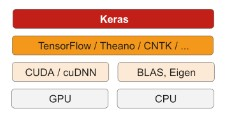
\includegraphics[width=6cm]{pictures/keras_layer.jpg}
  \caption{Hierarchical structure of Keras adapted from \cite{chollet_francois_2018}}
  \label{fig:keras_layer}
\end{figure}

\subsubsection*{TensorFlow}

TensorFlow \cite{DBLP:journals/corr/AbadiBCCDDDGIIK16} is the low-level framework that is used behind Keras \cite{moolayil_2019} for this thesis. It executes with dataflow graphs for computation representation, shared state, and with operations to mutate the state. Dataflow makes it possible to communicate between subcomputations and executing parallel independet computation. In TensorFLow all data is modelled as tensors which are $n$-dimensional arrays where each element have a small number of primitive datatypes. Furthermore, TensorFlow uses operations where one operation takes $m \geq 0$ inputs and computates $n \geq 0$ outputs.

\begin{figure}[ht!]
  \centering
  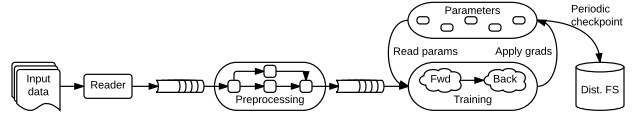
\includegraphics[width=11cm]{pictures/tensorflow_dataflow.jpg}
  \caption{TensorFlow dataflow graph that shows a training pipeline with subgraphs that take input data, preprocessing, training, and checkpointing state - adapted from \cite{DBLP:journals/corr/AbadiBCCDDDGIIK16}}
  \label{fig:tensorflow_dataflow}
\end{figure}

\subsection{Neural network}

A neural network (NN) \cite{Maas2013RectifierNI}, \cite{DBLP:journals/corr/ZhangZLS17} is a ML model which basis is a hierarchical neuron organization where the neurons are connected. In the neurons the computation for the output is executed.
The first layer are input data which are called tensors. Tensors are vectors in a n-dimensional matrix. The input data can be various types but only assigned as numeric data. The following example shows a $m x n$ shape which represents a two dimensional tensor (vector $a_{11}$ to $a_{m1}$ is one training sample):
\[
  A_{m\times n} =
  \left[ {\begin{array}{cccc}
    a_{11} & a_{12} & \cdots & a_{1n}\\
    a_{21} & a_{22} & \cdots & a_{2n}\\
    \vdots & \vdots & \ddots & \vdots\\
    a_{m1} & a_{m2} & \cdots & a_{mn}\\
  \end{array} } \right]
\]

The first hidden layer gets inputs from the input layer which receives the input data. The neurons in the hidden layer have a activation function which calculates the input data multiplied with weights.
Every ML model can have a stack of hidden layers one after another.

\begin{figure}[ht!]
  \centering
  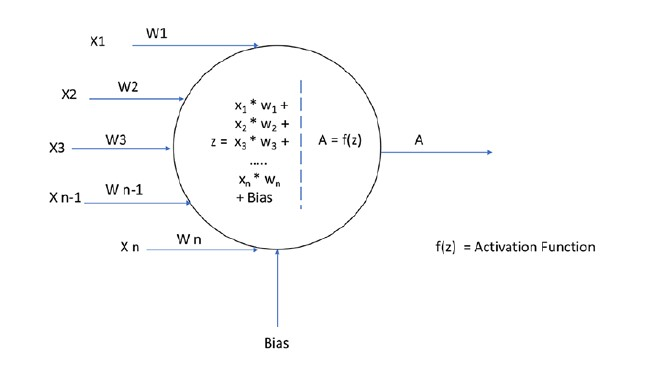
\includegraphics[width=10cm]{pictures/single_neuron.jpg}
  \caption{A single neuron adapted from \cite{moolayil_2019}.}
  \label{fig:single_neuron}
\end{figure}

The most common activation functions \cite{DBLP:conf/bmvc/Misra20} are the rectified linear unit (ReLU) function $Relu(z) = max(0, z)$ and the sigmoid function $\sigma(z) = \frac{1} {1 + e^{-z}}$ which are shown in Figure \ref{fig:sigmoid} and \ref{fig:relu}.

\begin{figure}[ht!]
  \centering
  \begin{minipage}[b]{0.4\textwidth}
    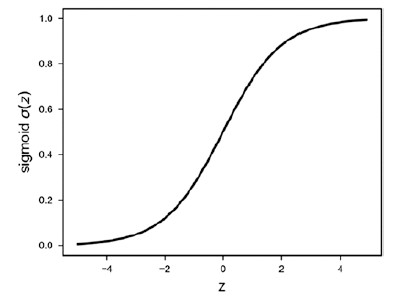
\includegraphics[width=6cm]{pictures/sigmoid.jpg}
    \caption{Sigmoid function adapted from \cite{moolayil_2019}}
    \label{fig:sigmoid}
  \end{minipage}
  \hfill
  \begin{minipage}[b]{0.4\textwidth}
    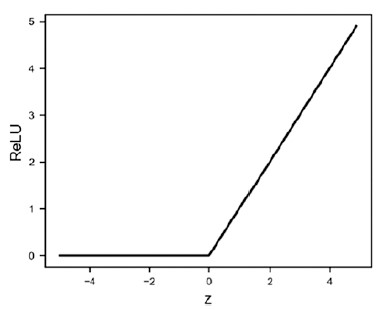
\includegraphics[width=6cm]{pictures/relu.jpg}
    \caption{ReLu function adapted from \cite{moolayil_2019}}
    \label{fig:relu}
  \end{minipage}
\end{figure}

After the hidden layers the NN has an output layer which shows the output as the name says. The next part of a NN is the loss function metric to measure the target loss. Popular loss functions \cite{DBLP:conf/cvpr/WanLC21} are the mean squared error $\sum_{i=1}^{D}(x_i-y_i)^2$ or the mean absolute error $\sum_{i=1}^{D}|x_i-y_i|$. \\ The main part of the ML model training is the optimizer which optimizes the ML model with an algorithm that is called backpropagation. Backpropagation executes after the ML model has started with the activation function and random weights in the defined structure explained earlier in this section. After this structure the loss function takes the ouput data to tell the NN how well it has predicted the input data based on the used weights. To update the weights for each neuron to reduce the loss, the optimizer algorithm uses a chain rule in calculus, derivates, and partial derivates. An example of an optimizer is stochastic gradient descent $Weights = Weights - learning rate * Loss$. The learning rate must be defined as a parameter in the NN architecture.

\begin{figure}[ht!]
  \centering
  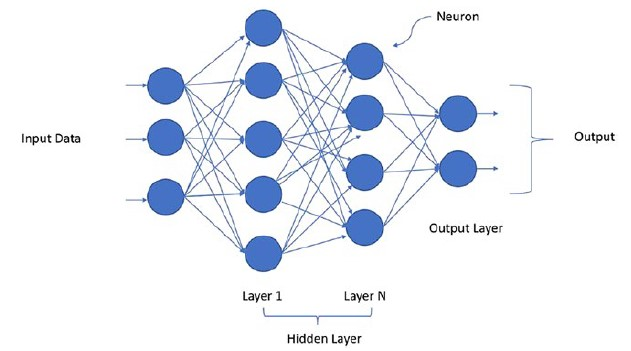
\includegraphics[width=10cm]{pictures/neural_network.jpg}
  \caption{NN example adapted from \cite{moolayil_2019}.}
  \label{fig:neural_network}
\end{figure}
